\section{Fundamentos}

\begin{frame}{¿Qué es el \textit{kernel} Linux?}
  \begin{itemize}
  \item Programa que \alert{ejecuta} programas y \alert{gestiona}
    dispositivos de hardware
  \item Encargado de que el software y el hardware puedan trabajar juntos
  \item Principales funciones
    \begin{itemize}
    \item Administración de \alert{memoria principal}
    \item Administración de \alert{uso de la CPU}
    \end{itemize}
  \item Es de código abierto a los usuarios \alert{(kernel/sched.c)}
  \item En una misma estructura de código fuente se da soporte a \alert{todass las arquitecturas}
  \item Liberado bajo licencia GPLv2  
  \item En un sentido estricto es el Sistema Operativo
  \end{itemize}
\end{frame}

\begin{frame}{¿Qué es el \textit{kernel} Linux?}
  \begin{itemize}
  \item Es un núcleo monolítico híbrido
    \begin{itemize}
    \item Los drivers y el código del Kernel se ejecutan en modo privilegiado
    \item Lo que lo hace híbrido es la posibilidad de cargar y descargar funcionalidad a través de módulos
    \end{itemize}
  \end{itemize}
  \vfill
  \pause
  \begin{block}{Software libre}
    Se dispone de la \alert{libertad} de: \vspace{-2ex}
    \begin{columns}[t]
      \column{0.4\textwidth}
      \begin{enumerate}
      \item Usar
      \item \textbf{Estudiar}
      \end{enumerate}
      \column{0.6\textwidth}
      \begin{enumerate}\addtocounter{enumi}{2}
      \item Distribuir
      \item Mejorar y publicar
      \end{enumerate}
    \end{columns}
  \end{block}
\end{frame}

\section{Historia}
\begin{frame}{Linux, un poco de historia}
  En 1991 Linus Torvalds inicia la programación del \textit{kernel} Linux
  basado en Minix\cite{Minix} (Clon de Unix desarrollado por Tanembaum en
  1987 con el fin de crear un SO de uso didáctico).

\begin{block}{Primer anuncio \hfill (1991)}\small
  \noindent Hello everybody out there using minix - 
 
  I’m doing a (free) operating system (just a hobby, won’t be big and
  professional like gnu) for 386(486) AT clones.

  [\ldots]
  
  It is \alert{NOT protable} (uses 386 task switching etc), and it probably never
  will support anything other than AT-harddisks, as that’s all I have :-(.\\
  
  \hfill \emph{Linus Torvalds}, 25/08/1991, \texttt{\small
    comp.os.minix\cite{Torvalds1992}}
\end{block}

% \item Desarrollo continuado por miles de programadores alrededor del mundo
\end{frame}

\begin{frame}{Linux, un poco de historia}
El 5 de octubre de 1991, se anuncia la primera versión ``oficial'' de
Linux (0.02).

\begin{block}{Primera \textit{release} \hfill (1991)}
  [\ldots]

  As I mentioned a month ago, I'm working on a free version of a
  minix-lookalike for AT-386 computers. It has finally reached the stage
  where it's even usable (though may not be depending on what you want),
  and I am willing to put out the sources for wider distribution. It is
  just version 0.02 (+1 (very small) patch already), but I've successfully
  run bash/gcc/gnu-make/gnu-sed/compress etc under it.

  [\ldots]

  \hfill \emph{Linus Torvalds}, 05/10/1991, \texttt{\small
    comp.os.minix\cite{Torvalds1992}}

\end{block}
\end{frame}

\begin{frame}{Linux, un poco de historia}
  \small En 1992, con la \textit{release} de la versión 0.12, se decide
  cambiar a una licencia GNU.

\begin{block}{Licencia GNU \hfill (1992)}
  {\small

  [\ldots]

  The Linux copyright will change: I've had a couple of requests to make it
  compatible with the GNU copyleft, removing the ``you may not distribute
  it for money'' condition.  I agree.  I propose that the copyright be
  changed so that it confirms to GNU - pending approval of the persons who
  have helped write code.  I assume this is going to be no problem for
  anybody: If you have grievances (``I wrote that code assuming the
  copyright would stay the same'') mail me.  Otherwise The GNU copyleft
  takes effect as of the first of February.  If you do not know the gist of
  the GNU copyright - read it.

  [\ldots]

  }

  \hfill \emph{Linus Torvalds}, 1992 \cite{Torvalds1992-2}
\end{block}
\end{frame}

\begin{frame}{Linux, un poco de historia}
Fechas relevantes:
\begin{itemize}
\item En marzo de 1994 Torvalds considera que todos los componentes del
  \textit{kernel} estaban suficientemente maduros y lanza la versión 1.0.

\item En el año 1995 Linux se porta a arquitecturas \textit{DEC Alpha} y
  \textit{Sun SPARC}. Con el correr de los años se portó a otra decena de
   arquitecturas.

\item En mayo de 1996 se decide adoptar a Tux como mascota oficial de
  Linux.
\end{itemize}
\end{frame}

\begin{frame}{Linux, un poco de historia}
Fechas relevantes:
  \begin{itemize}
\item En julio de 1996 se lanza la versión 2.0 y se define un sistema de
  nomenclatura. Se desarrolló hasta febrero de 2004 y terminó con la
  versión 2.0.40. Esta versión comenzó a brindar soporte a sistemas
  multiprocesadores.

\item En 2001 se lanza la versión 2.4 y se deja de desarrollar a fines del
  2010 con la 2.4.37.11. La versión 2.4 fue la que catapultó a GNU/Linux
  como un sistema operativo estable y robusto.
\end{itemize}
\end{frame}

\begin{frame}{Linux, un poco de historia}
Fechas relevantes:
\begin{itemize}
\item A fines del año 2003 se lanza la versión 2.6. Esta versión ha tenido
  muchas mejoras para el \textit{kernel} dentro de las que se destacan
  soporte de \textit{threads}, mejoras en la planificación y soporte de
  nuevo hardware.

\item El 3 de agosto de 2011 se lanza la versión 2.6.39.4 anunciándose la
  misma desde meses previos como la última en su revisión.

\item El 17 Julio de 2011 se lanza la versión 3.0
    \begin{itemize}
    \item No agrega mayores cambios. La decisión del cambio son los 20 años del SO y no superar los 40 números de revisión
    \item Totalmente compatible con Kernel 2.6
    \end{itemize}

\end{itemize}
\end{frame}

\begin{frame}{Linux, un poco de historia}
\begin{itemize}
\item El 17 Julio de 2011 se lanza la versión 3.0
    \begin{itemize}
    \item Termina con la versión 3.8.30
    \item Provee mejoras en Virtualización y FileSystems
    \end{itemize}
\end{itemize}

\begin{block}{Anuncio de Linux 3.0 \hfill (2011)}
  [\ldots]

  I decided to just bite the bullet, and call the next version 3.0. It will
  get released close enough to the 20-year mark, which is excuse enough for
  me, although honestly, the real reason is just that I can no longer
  comfortably count as high as 40.

  [\ldots]

  \hfill \emph{Linus Torvalds},  2011 \cite{Torvalds2011}
\end{block}
\end{frame}

\begin{frame}{Linux, un poco de historia}
\begin{itemize}
\item El 12 de Abril de 2015 se lanza la versión 4.0
    \begin{itemize}
    \item Una de sus principales mejoras es la posibilidad de aplicar parches y actualizaciones si necesidad de reiniciar el SO.
    \item Soporte para nuevas CPU
    \item La versión actual es 4.5
    \end{itemize}
\end{itemize}

\begin{block}{Anuncio de Linux 4.0 \hfill (2015)}
  [\ldots]

  .. Because the people have spoken, and while most of it was complete
gibberish, numbers don't lie. People preferred 4.0, and 4.0 it shall
be. Unless somebody can come up with a good argument against it.

  [\ldots]

  \hfill \emph{Linus Torvalds},  2015
\end{block}
\end{frame}


\section{Versionado}
\begin{frame}{Versionado en Linux 2.6 y 3/4}
  
  \begin{block}{Anatomía de una versión}
    \alert{A}.\alert{B}.\structure{C}.[\structure{D}]
  \end{block}

    { \tiny
  \begin{description}

  \item[\alert{A}] Denota Versión. Cambia con menor Frecuencia. en 1994
    (versión 1.0), en 1996 (versión 2.0), en 2011 (versión 3.0) y en  en 2015 (versión 4.0).

  \item[\alert{B}] Denota revisión mayor. Antes de la versión 2.6, los
    números impares indicaban desarrollo, los pares producción.

  \item[\structure{C}] Denota revisión menor. Solo cambia cuando hay nuevos
    \textit{drivers} o características.

  \item[\structure{D}] Se utiliza cuando se corrige un grave error sin
    agregar nueva funcionalidad.
  \end{description} }

  \vfill \pause En el año 2011, cuando se pasó de la versión
  \alert{2}.\alert{6}.\structure{39} a la \alert{3}.\structure{0}, se
  eliminó el número de revisión mayor (\alert{B})\cite{Torvalds2011}.

\end{frame}

\begin{frame}{Versionado previo a la versión 2.6}
  \begin{block}{Anatomía de una versión}
    \alert{X}.\alert{Y}.\structure{Z}
  \end{block}
  \begin{description}

  \item[\alert{X}] Indica serie principal. Cambia cuando su funcionalidad
    sufre un cambio muy importante.

  \item[\alert{Y}] Indica si es una versión de producción o desarrollo.
  \item[\structure{Z}] Nuevas versiones dentro de la
    actual. \textit{Bugfixes}.
  \end{description}
  \begin{itemize}
  \item Existían dos versiones del \textit{kernel}:
    \begin{itemize}
    \item Números \alert{Y} pares indicaban versión en Producción (estable)
    \item Números \alert{Y} impares indicaban versión en Desarrollo
    \end{itemize}    
  \end{itemize}
\end{frame}

\section{Compilación}
\begin{frame}{¿Por qué recompilarlo?}
\begin{itemize}
\item Soportar \alert{nuevos dispositivos} como, por ejemplo, una placa de
  video

\item Agregar \alert{mayor funcionalidad} (soporte para algún hardware
  específico)

\item Optimizar funcionamiento de acuerdo al \alert{sistema en el que
    corre}

\item \alert{Adaptarlo} al sistema donde corre (quitar soporte de hardware no utilizado)

\item \alert{Corrección} de \textit{bugs} (problemas de seguridad o errores de programación)
\end{itemize}
\end{frame}

\begin{frame}{¿Qué necesitamos?}
\begin{itemize}
\item \texttt{gcc}: Compilador de C

\item \texttt{make}: ejecuta las directivas definidas en los
  \texttt{Makefiles}
\item \texttt{binutils}: \textit{assembler}, \textit{linker}
\item \texttt{libc6}: Archivos de encabezados y bibliotecas de desarrollo
\item \texttt{ncurses}: bibliotecas de menú de ventanas (solo si usamos
  \texttt{menuconfig})
\item \texttt{initrd-tools}: Herramientas para crear discos RAM
\end{itemize}
\pause
\begin{block}{Tip}
  En Debian y distribuciones derivadas, todo este software se encuentra
  empaquetado. Por ejemplo, para instalar el software requerido para hacer
  la práctica:

  \texttt{\# apt-get install build-essentials libncurses-dev}
\end{block}
\end{frame}

\begin{frame}{Proceso de compilación de Linux}
\begin{enumerate}
\item Obtener el código fuente.
\item Preparar el árbol de archivos del código fuente.
\item Configurar el \textit{kernel}
\item Construir el \textit{kernel} a partir del código fuente e instalar los
  módulos.
\item Reubicar el \textit{kernel}.
\item Creación del \texttt{initramfs}
\item Configurar y ejecutar el gestor de arranque (LILO, GRUB, etc).
\item Reiniciar el sistema y probar el nuevo kernel.
\end{enumerate}
\end{frame}

\begin{frame}{Obtener el código fuente}
  \large \url{http://www.kernel.org}
  \begin{center}
    \fbox{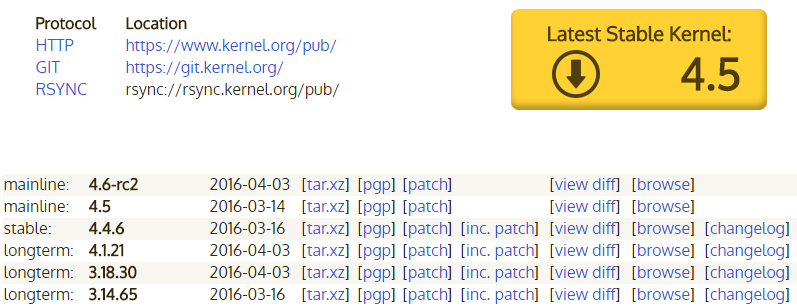
\includegraphics[width=0.8\textwidth]{../../../common/images/kernelorg-homepage}}
   \end{center}
\end{frame}

\begin{frame}{Obtener el código fuente}
  Para descargarlo desde la terminal:
  \begin{block}{}
    \tiny {
    \texttt{\$ cd /usr/src}\\
    \texttt{\$ sudo wget
      https://kernel.org/pub/linux/kernel/v4.x/linux-\KERNELBASEVERSION.tar.xz} }
  \end{block}	
  \vfill
  \alert{Opcional}: Por cuestiones de seguridad, opcionalmente se puede
  descargar un archivo con una firma criptográfica del \textit{kernel}
  descargado. Esta firma nos permite comprobar que el archivo que
  descargamos es exactamente el mismo que fue subido, y que no hubo
  modificaciones maliciosas de por medio.
  \begin{block}{}
    \tiny{\texttt{%
\$ wget https://kernel.org/pub/linux/kernel/v4.x/linux-\KERNELBASEVERSION.tar.sign \\
\$ xz -cd linux-\KERNELBASEVERSION.tar.xz | gpg --verify linux-\KERNELBASEVERSION.tar.sign -\\
gpg: Signature made Thu 30 Mar 2014 11:35:06 AM ART using RSA key ID 4395693E\\
gpg: Good signature from ``Greg Kroah-Hartman (Linux kernel stable release signing key) <greg@kroah.com>''\\
gpg: WARNING: This key is not certified with a trusted signature!\\
gpg:          There is no indication that the signature belongs to the owner.\\
Primary key fingerprint: 647F 2865 4894 E3BD 4571  99BE 38DB BDC8 6092 693E}}
\end{block}
    
\end{frame}

\begin{frame}{Preparar el árbol de archivos}
  Por convención el código fuente del \textit{kernel} se guarda en
  \texttt{/usr/src}. Sin embargo, como dicho directorio generalmente no
  tiene permisos de escritura para usuarios no privilegiados, el archivo se
  debe descomprimir en un directorio donde tengamos permisos, como el
  \texttt{\$HOME} del usuario actual.
  { \small
  \begin{block}{}
    \texttt{\$ mkdir \KERNELSOURCEPATH}\\
    \texttt{\$ cd \KERNELSOURCEPATH}\\
    \texttt{\$ tar xvf /usr/src/linux-\KERNELBASEVERSION.tar.xz}
  \end{block}}
  Generalmente se crea un enlace simbólico llamado linux apuntando al directorio del código fuente que actualmente se está configurando
  \begin{block}{}
    \texttt{\$ ln -s /usr/src/linux-\KERNELBASEVERSION\   /usr/src/linux}
  \end{block}

\end{frame}

\begin{frame}{Configurar el \textit{kernel}}
  El \textit{kernel} Linux se configura mediante el archivo
  \texttt{.config}. Este archivo, que reside en la raíz del directorio del
  \textit{kernel}, contiene las instrucciones de qué es lo que el
  \textit{kernel} debe compilar.

  \begin{block}{}
    \tiny {
    \texttt{%
\$ cat /boot/config-\$(uname -r) | tail -n5 \\
CONFIG\_UCS2\_STRING=y \\
CONFIG\_FONT\_SUPPORT=y \\
\# CONFIG\_FONTS is not set \\
CONFIG\_FONT\_8x8=y \\
CONFIG\_FONT\_8x16=y}}
  \end{block}
\pause
Existen tres interfaces que permiten generar este archivo:
\begin{itemize}
\item \texttt{make config}: modo texto y secuencial. \alert{Tedioso}.
\item \texttt{make xconfig}: interfaz gráfica utilizando un sistema de
  ventanas.\alert{No todos los sistemas tienen instalado X}.
\item \texttt{make menuconfig}: este modo utiliza \texttt{ncurses}, una
  librería que permite generar una interfaz con paneles desde la terminal.\alert{Generalmente el más utilizado}.
\end{itemize}
\end{frame}

\begin{frame}{Configurar el \textit{kernel}}
Las herramientas mencionadas permiten:
\begin{itemize}
\item Crear un archivo \texttt{.config} con las directivas de compilación
\item Configurar un \textit{kernel} desde cero es una tarea tediosa y
  propensa a errores (\textit{kernels} que no arranquen). Estas
  herramientas automatizan el proceso por nosotros.
\end{itemize}

\begin{block}{Consejos}
\begin{itemize}
\item Lo ideal es ir manteniendo el \texttt{.config} para no tener que
  configurar todo de cero

\item Cada nueva versión, puede valerse de un \texttt{.config} anterior.

\item Por convención, es recomendable almacenar en el directorio
  \texttt{/boot} la imagen compilada del \textit{kernel} junto con su
  \texttt{.config}.
\end{itemize}
\end{block}
\end{frame}

\begin{frame}{Configurar el \textit{kernel} (Modulos)}
¿Qué es un modulo del Kernel?
\begin{itemize}
\item Un fragmento de código que puede cargarse/descargarse en el mapa de memoria del SO (Kernel)bajo demanda
\item Permiten extender la funcionalidad del Kernel en ``caliente'' (sin necesidad de reiniciar el sistema
\item Todo su codigo se ejecuta en modo Kernel (privilegiado)
\item Cualquier error en el módulo, puede colgar el SO
\item Permiten que el kernel se desarrolle bajo un diseño mas modular
\item Los modulos disponibles se ubican en \textit{/lib/modules/version del kernel}
\item Con el comando \textit{lsmod} es posible ver qué modulos están cargados
\item \alert{Vamos a ampliar en las próximas prácticas}
\end{itemize}
\end{frame}


\begin{frame}{Configurar el \textit{kernel}}
¿El soporte lo damos como módulo o \textit{built-in}?
\pause
\begin{itemize}
\item Si es \textit{built-in}, el kernel crece. Más ocupación en memoria, más lento el arranque
\item Si es \textit{built-in}, es mas eficiente su utilización. No hay que
  cargar un adicional en memoria, acceso directo.
\item En el soporte como módulo:
  \begin{itemize}
  \item Si se quiere dar soporte a algún dispositivo, se carga el módulo y
    no es necesario recompilar (el soporte debe estar en el
    \textit{kernel}).

  \item Si hay una modificación de un \textit{driver}, solo se modifica el
    módulo y no todo el código del \textit{kernel}.

  \item Los módulos se cargan bajo demanda, con lo cual la utilización de
    memoria es menor.
  \end{itemize}
\end{itemize}
\end{frame}

\begin{frame}{Parcheando el \textit{kernel}}
\begin{itemize}
\item Es un mecanismo que permite aplicar actualizaciones NO incrementales sobre la version base
\item Se basa en archivos \textit{diff} (archivos de diferencia), que indican qué agregar y qué quitar
\item Se aplican sobre la versión base
\item Permiten agregar funcionalidad (nuevos drivers, correcciones menores, etc.)
\item A veces puede resultar más sencillo descargar el archivo de diferencia y aplicarlo en vez de descargar todo el código de la nueva versión
\end{itemize}
\pause
\begin{block}{}
    \texttt{\$ cd linux; zcat ../patch-\PATCHEDKERNELVERSION.gz | patch -p1}
\end{block}

\begin{block}{Tip}
  Parámetro útil:
  \texttt{\ --dry-run}
\end{block}

\end{frame}


\begin{frame}{Configurar el \textit{kernel}}
  En el trabajo práctico debemos dar el siguiente soporte adicional:
  \begin{itemize}

  \item Soporte para \textbf{FS Minix}: En la opción \textit{File Systems}
    $\to$ \textit{Miscellaneous filesystems}, tendremos que seleccionar
    \textit{Minix fs support}

  \item Soporte para \textbf{FS ext4}: En la opción \textit{File Systems},
    tendremos que seleccionar \textit{The Extended 4 (ext4) filesystem}

  \item Soporte para dispositivos de \textbf{Loopback}: En la opción
    \textit{Device Drivers} $\to$ \textit{Block Devices}, tendremos que
    seleccionar \textit{Loopback device support}.
  \end{itemize}
\end{frame}

\begin{frame}{Compilación del \textit{kernel}}
\begin{block}{}
  \texttt{\$ make} 
\end{block}
El comando \texttt{make} busca el archivo \texttt{Makefile}, interpreta sus
directivas y compila el \textit{kernel}. Este proceso puede durar mucho
tiempo dependiendo del procesador que tengamos.

\begin{block}{Tip}
\texttt{\$ make -j\textit{X} \# X es el número de \textit{threads}}
\end{block}

Verificar que este proceso no arroje errores al concluir.
\end{frame}

\begin{frame}{Compilando}
  \large XKCD \#303 \\ \url{http://xkcd.com/303/}
  \begin{center}
    \fbox{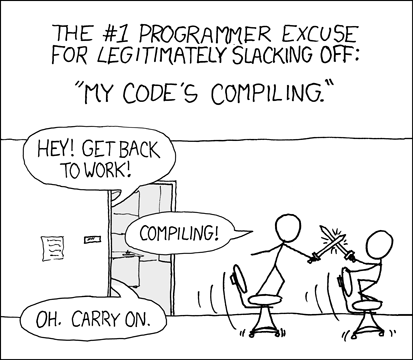
\includegraphics[width=0.4\textwidth]{../../../common/images/compiling}}
   \end{center}
\end{frame}

\begin{frame}{Compilación de \textit{modulos}}
\begin{block}{Compilando}
  \texttt{\$ make modules} 
\end{block}

El comando \texttt{make modules} compila todos los módulos necesarios para satisfacer las opciones que hayan sido seleccionadas como módulo .

\begin{block}{Tip}
\texttt{Generalmente la tarea anterior se encuentra incluida en la compilación del kernel con el comando \texttt{make}}
\end{block}


\end{frame}


\begin{frame}{Instalación del \textit{kernel}}
  \alert{Recién en este paso es necesario convertirse en root}

  Al terminar el proceso de compilación, la imagen del
  \textit{kernel} quedará ubicada en
  \texttt{\textit{directorio-del-código}/arch/\textit{arquitectura}/boot/}. El
  próximo paso, entonces, es instalar el \textit{kernel} y otros archivos
  en el directorio \texttt{/boot}.

  { \tiny
  \begin{block}{Ejemplo con arquitectura \textit{i386}}
    \texttt{\$ cd \KERNELSOURCEPATH/linux-\KERNELVERSION \\
\$ sudo su \\
\# cp arch/i386/boot/bzImage /boot/vmlinuz-\PATCHEDKERNELVERSION \\
\# cp System.map /boot/System.map-\PATCHEDKERNELVERSION \\
\# cp .config /boot/config-\PATCHEDKERNELVERSION}
  \end{block}}
  \vfill \pause

\tiny
  Por supuesto, también existe una regla en el \texttt{Makefile} que
  realiza esto mismo automáticamente.
  { \tiny
  \begin{block}{}
    \texttt{\$ sudo make install}
  \end{block}}
System.map: http://rlworkman.net/system.map/
\end{frame} 

\begin{frame}{Instalar los módulos}
  Los módulos compilados deben residir en el directorio
  \texttt{/lib/modules/\textit{version-del-kernel}}. Al igual que en el
  paso anterior, el archivo \texttt{Makefile} tiene una regla para instalar
  los módulos.
  \begin{block}{}
    \texttt{\$ sudo make modules\_install}
  \end{block}
  El parámetro \texttt{modules\_install} es una regla del \texttt{Makefile}
  que ubica los módulos del \textit{kernel} recién compilado en el
  directorio correspondiente.
\end{frame}

\begin{frame}{Creación del \texttt{initramfs}}
  Un \texttt{initramfs} es un sistema de archivos temporal que se monta
  durante el arranque del sistema. Contiene ejecutables, \textit{drivers} y
  módulos necesarios para lograr iniciar el sistema. Luego del proceso de
  arranque el disco se desmonta.
  
  \begin{block}{}
    \texttt{\# mkinitramfs -o /boot/initrd.img-\PATCHEDKERNELVERSION\ \PATCHEDKERNELVERSION }
  \end{block}  
\end{frame}

\begin{frame}{Configuración del gestor de arranque}
\begin{itemize}
\item \texttt{LILO}
  \begin{block}{\texttt{/etc/lilo.conf}}
    \texttt{image=/boot/vmlinuz-\PATCHEDKERNELVERSION \\
    label=Linux-kernel-\PATCHEDKERNELVERSION \\
    read-only \\
    root=/dev/sda1}
  \end{block}
\item GRUB \textit{legacy}
  \begin{block}{\texttt{/boot/grub/menu.lst}}
    \texttt{title     Linux-kernel-\PATCHEDKERNELVERSION \\
    root     (hd0,0) \#Disco en el 1º IDE, 1º partición \\
    kernel  /vmlinuz-\PATCHEDKERNELVERSION\ root=/dev/sda1 ro \\
    initrd /initrd.img-\PATCHEDKERNELVERSION}
  \end{block}
\end{itemize}
\end{frame}
\begin{frame}{Configuración del gestor de arranque}
  En el trabajo práctico utilizaremos la versión 2 de GRUB. Luego de
  instalar el \textit{kernel}, para que el gestor de arranque lo reconozca
  simplemente deberemos ejecutar, como usuario privilegiado, el siguiente
  comando:

  \begin{block}{}
    \texttt{\# update-grub2}
  \end{block}
  
\end{frame}

\begin{frame}{Finalización del proceso}

Verificar que el \textit{kernel} esté instalado en \texttt{/boot}:

{ \tiny
  \begin{block}{}
    \texttt{\$ test -f /boot/vmlinuz-\PATCHEDKERNELVERSION\ \&\& echo ``Kernel instalado''}
\end{block} }

Verificar que los módulos estén instalados en
\texttt{/lib/modules/\PATCHEDKERNELVERSION}:

{ \tiny
  \begin{block}{}
    \texttt{\$ test -d /lib/modules/\PATCHEDKERNELVERSION-\textit{arquitectura}
      \&\& echo ``Modulos aparentemente instalados''}
\end{block} }

Verificar que el gestor de arranque haya indexado el \textit{kernel}. Si el
gestor de arranque utilizado es GRUB 2, entonces el siguiente comando
debería generar un par de líneas de salida.

  { \tiny
  \begin{block}{}
    \texttt{\$ cat /boot/grub/grub.cfg  | grep --color \KERNELBASEVERSION}
\end{block} }

Paso final: ¡\alert{reiniciar} y \structure{probar}!
\end{frame}

\section{Apéndice}

\subsection{Debian way}
\begin{frame}{Debian \textit{way}}
Instalar un \textit{kernel} de forma empaquetada ofrece muchas ventajas:
\begin{itemize}
\item Integración con el sistema operativo
\item \textit{Bugfixes}
\item Actualizaciones de \alert{seguridad}
\item LTS (\textit{Long Term Support})
\end{itemize}

\vfill Debian designa una versión de Linux a la cual dar soporte durante
todo el ciclo de vida de su versión estable, actualmente Debian
\textit{jessie}. Esto implica portar actualizaciones críticas y
\textit{bugfixes}. La versión de Linux que está en la actual Debian estable
es la 3.16.

{ \tiny
  \begin{block}{}
    \texttt{\\
\# apt-get install linux-source-3.16 \\
\$ tar xjf /usr/src/linux-source-3.16.tar.bz2 \\
\$ cd linux-source-3.16 \\
\$ make menuconfig \\
\$ scripts/config --disable DEBUG\_INFO \\
\$ make clean \\
\$ make deb-pkg \\
\# dpkg -i ../linux-image-3.16.*.deb
}
\end{block} }

\end{frame}

\begin{frame}{Referencias}
  \begin{thebibliography}{Foo Bar Baz, 1968}\footnotesize
  \bibitem{Torvalds2011} Linus Torvalds \newblock {\em Linux 3.0-rc1}
    \newblock \url{https://lkml.org/lkml/2011/5/29/204}, 2011
  \bibitem{Minix} Andrew Tanembaum \newblock {\em Minix} \newblock
    \url{http://www.minix3.org/}
  \bibitem{Torvalds1992} Linus Torvalds \newblock {\em Linux History} \newblock
    \url{https://www.cs.cmu.edu/~awb/linux.history.html}, 1992
  \bibitem{Torvalds1992-2} Linus Torvalds \newblock {\em Release notes for Linux v0.12} \newblock
    \url{http://ftp.funet.fi/pub/linux/historical/kernel/old-versions/RELNOTES-0.12}, 1992
  \bibitem{DebianKernelHandboox} \newblock {\em Debian Linux Kernel Handbook}
    \newblock \url{http://kernel-handbook.alioth.debian.org/}
  \end{thebibliography}
\end{frame}

\begin{frame}[fragile]
\frametitle{DESAFIO}
   \begin{itemize}  
   \item Compilar el Kernel en la distribución que posean
   \item Una vez que el kernel haya sido compilado, bootear con ese kernel y ejecutar el siguiente comando:
   \begin{lstlisting}
# uname -r | md5sum
    \end{lstlisting}
    \item Pegar el texto devuelto en la tarea que se publicará para tal fin en el sitio de la cátedra
    \item ¡Tienen tiempo hasta el Lunes 18 a las 15:00 horas!
 \end{itemize}
\end{frame}

%%% Local Variables: 
%%% mode: latex
%%% TeX-master: "main"
%%% End:
